\input{../.preambles/03-questions}
\input{../.preambles/10-russian}
\input{../.preambles/20-math}

\newcommand{\up}{\uparrow}
\newcommand{\down}{\downarrow}
\newcommand{\updown}{\up\down}
\newcommand{\ds}{\displaystyle}
\renewcommand{\i}{\mathrm{i}}
\newcommand{\e}{\mathrm{e}}

\begin{document}
\def\contentsname{Список вопросов}
\tableofcontents
\newpage
\question{Предмет квантовой электроники. История возникновения и развития
квантовой электроники. Современные достижения и возможности квантовой
электроники}

\subquestion{Предмет квантовой электроники}

\emph{Квантовая электроника} -- это область физики, изучающая методы усиления
и генерации электромагнитного излучения путём использования эффекта
вынужденного излучения в термодинамически неравновесных квантовых системах,
свойства получаемых таким образом генераторов и усилителей и их применения.
Другими словами, это наука о мазерах и лазерах.

\subquestion{Фундаментальные физические предпосылки создания квантовой
электроники}
\begin{enumerate}
    \item[1900 г.] Планк получил верный результат для теплового излучения исходя
        из квантов излучения
    \item[1905 г.] Эйнштейн пришёл к гипотезе световых квантов
    \item[1913 г.] Бор связал частоту излучения с разностью уровней энергии
    \item[1916 г.] Эйнштейн вывел формулу Планка, постулировав вынужденное
        излучение
    \item[1924 г.] Бозе и Эйнштейн получили статистику Бозе-Эйнштейна, которой
        подчиняются фотоны
    \item[1927 г.] Дирак строго обосновал существование вынужденного излучения
        и его свойства
\end{enumerate}

\subquestion{История возникновения и развития}
\begin{enumerate}
    \item[1954 г.] -- были даны непосредственные теоретические основы
        квантовой электроники и создан первый прибор -- пучковый аммиачный
        мазер
    \item[1955 г.] -- Басов и Прохоров предложили трёхуровневый метод накачки
    \item[1960 г.] -- первый лазер (рубиновый, гелий-неоновый)
    \item[1962 г.] -- полупроводниковый лазер
    \item[1964 г.] -- молекулярный \( \mathrm{CO_2} \) лазер
\end{enumerate}

\subquestion{Современные достижения и возможности квантовой электроники}
На сегодняшний день лазеры позволяют получать импульсы до 10~МВт длительностью
от 10~нс до микросекунд (с помощью модуляции добротности можно получить и
фемтосекунды) интенсивностью до 1~ТВт/\(\text{см}^2\). КПД при этом может
достигать 15\%.

Области применения лазеров:
\begin{itemize}
    \item научно исследовательская деятельность
    \item промышленность
    \item термические технологии (сварка, резка, скрабирование)
    \item для разделения изотопов
    \item для оптического контроля
    \item для связи (оптоволокно, атмосфера)
    \item в медицине
\end{itemize}


\chapter{Математическая модель теплопроводности. Некоторые уравнения
диффузионного типа.}

Математическая модель теплопроводности представляет собой систему четырех
уравнений:
\[
    \left. \begin{array}{rl}
        \text{ДУЧП:} & \ds \pder{u}{t} = \alpha^2\ppder{u}{x}, 
        \vspace*{.4em} \\
        \text{ГУ:} & \left\{ \begin{array}{l}
            u(0, t) = f_1(t), \\
            u(l, t) = f_2(t), 
        \end{array} \right. \\
        \text{НУ:} & u(x, 0) = \phi(x).
    \end{array} \right\}
\]

\section{Некоторые уравнения диффузионного типа:}
\begin{enumerate}
    \item теплообмен через боковую поверхность, пропорциональный разности
    температур:
    \[
        \pder{u}{t} = \alpha^2\ppder{u}{x} - \beta(u - u_0);
    \]
    
    \item внутренний источник тепла:
    \[
        \pder{u}{t} = \alpha^2\ppder{u}{x} + f(x, t);
    \]
    
    \item уравнение конвективной диффузии:
    \[
        \pder{u}{t} = \alpha^2 \ppder{u}{x} - v\pder{u}{x}.
    \]
\end{enumerate}

\newpage % ---------------------------------------------------------------------

\question{Спонтанные и индуцированные переходы. Коэффициенты Эйнштейна.}

При индуцированных переходах квантовая система может переводиться из одного 
энергетического состояния в другое \ref{img1.1} как с поглощение энергии 
электромагнитного поля (переход с нижнего на верхний), так и с излучением 
электромагнитной энергии (переход с верхнего на нижний).

\begin{figure}[h!]
	\center
	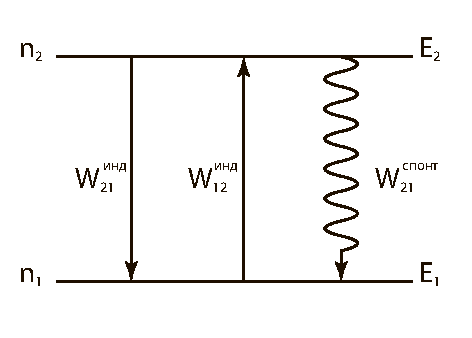
\includegraphics[width=.4\textwidth]{image1_1} \\
	\caption{Схема двух уровней энергии \( E_2 > E_1 \)}
	\label{img1.1}
\end{figure}

Индуцированные переходы обладают следующими важными свойствами.

Во-первых, вероятность индуцированных переходов отлична от нуля только для 
внешнего поля резонансной частоты, энергия которого \( h\nu \) совпадает с 
разностью энергий двух изолированных состояний (\( E_2 \) и \( E_1 \), где 
индекс 2 относится к большей энергии, а 1 -- к меньшей). Это условие 
соответствия постулату Бора:
\[
	h\nu = E_2 - E_1
\]

Во-вторых, кванты электромагнитного поля, излученные при индуцированных 
переходах, полностью тождественны квантам поля, вызвавшего эти переходы. 
То есть внешнее электромагнитное поле и поле, созданное при индуцированных 
переходах, имеют одинаковые частоту, фазу, поляризацию и направление 
распространения -- они тождественны.

В-третьих, вероятность индуцированных переходов в единицу времени 
пропорциональна плотности энергии внешнего поля в единичном спектральном 
интервале:
\[
	W_{12}^\text{инд} = B_{12}\rho_\nu
\]
\[
	W_{21}^\text{инд} = B_{21}\rho_\nu
\]

где \( B_{12} \) и  \( B_{21} \) -- коэффициенты Эйнштейна для индуцированного 
поглощения и излучения соответственно, а порядок индексов 1 и 2 указывает 
направление перехода.

Таким образом индуцированное излучение -- это излучение вынужденное, 
стимулированное внешним излучением. 

Кроме индуцированного внешним полем, существует и самопроизвольное испускание 
излучения. Атомы, находящиеся в верхнем энергетическом состоянии, могут 
совершать спонтанные переходы в нижнее состояние. Эти переходы 
самопроизвольны. Происходящий при спонтанном излучении распад верхнего 
энергетического состояния подобен радиоактивному распаду неустойчивого ядра. 
Вероятность спонтанных переходов не зависит от внешнего электромагнитного 
поля, акты спонтанного излучения никак не связаны с внешним полем. Поэтому 
спонтанное излучение некогерентно по отношению к внешнему полю и играет 
роль собственных шумов. Кроме того, спонтанное излучение опустошает верхний 
энергетический уровень, способствуя возвращению атома в нижнее энергетическое 
состояние.

Спонтанное излучение является эффектом принципиально квантовым, не допускающим 
классической трактовки. В классической механике метастабильное состояние, 
обладающее большей энергией по отношению к некоторому основному устойчивому 
состоянию, в отсутствие внешних возмущений может жить бесконечно долго. В 
квантовой области такое метастабильное состояние спонтанно распадается с 
некоторой отличной от нуля средней скоростью.

Рассмотрим ансамбль квантовых частиц, находящихся в термостате при 
температуре \( T \). Пусть рассматриваемая квантовая система обладает двумя 
уровнями энергии \( E_2 > E_1 \), при переходах между которыми поглощается 
или излучается квант энергии \( h\nu \). При термодинамическом равновесии 
ансамбль не теряет и не приобретает энергии. Следовательно, в единицу времени 
во всём ансамбле общее число переходов из верхнего энергетического состояния 
в нижнее должно быть равным общему числу переходов из нижнего состояние в 
верхнее. Общее число переходов определяется числом частиц на уровнях энергии 
или населенностью уровней. 

При тепловом равновесии распределение частиц по уровням подчиняется формуле 
Больцмана:
\[
	\frac{n_2}{g_2} = \frac{n_1}{g_1}\exp
		\left[ -\frac{E_2 - E_1}{kT}\right]
\]
где \( g_2 \) и \( g_1 \) -- кратность вырождения уровней 2 и 1, 
\( k \) -- постоянная Больцмана.

Полное число переходов \( 2 \rightarrow 1 \) равно произведению числа частиц 
\( n_2 \) в состояние \( 2 \) на вероятность перехода \( 2 \rightarrow 1 \) 
в единицу времени для одной частицы. Вероятность самопроизвольного перехода 
частицы из верхнего состояния в нижнее пропорциональна времени. За время 
\( dt \) эта вероятность составляет по предположению
\[
	dw^\text{спонт} = A_{21} dt
\]
где \( A_{21} \) -- коэффициент Эйнштейна для спонтанного излучения. Таким 
образом вероятность спонтанного испускания излучения в единицу времени 
постоянна и равна по определению соответствующему коэффициенту Эйнштейна 
\( A_{21} \):
\[
	W_{21}^\text{спонт} = A_{21}
\]

Частицы рассматриваемого ансамбля находятся в поле их собственного излучения, 
плотность энергии которого в единичном спектральном интервале составляет 
\( \rho_\nu \). Это поле индуцирует переходы из верхнего состояния в нижнее 
и обратно. Вероятности этих переходов пропорциональны \( \rho_\nu \). 
Комбинируя предыдущие формулы, можем из условия равновесия
\[
	g_1 B_{12} \rho_\nu \exp\left[ -\frac{E_1}{kT} \right] = 
	g_2 \left( B_{21}\rho_nu + A_{21} \right)
		\exp\left[ -\frac{E_2}{kT} \right]
\]
найти соотношения между коэффициентами \( A_{21}, B_{12}, B_{21} \). Это 
уравнение позволяет легко найти плотность энергии поля излучения 
рассматриваемой равновесной квантовой системы:
\[
	\rho_\nu = \frac{A_{21}}{B_{21}}
		\left[ 
			\frac{g_1 B_{12}}{g_2 B_{21}}\exp\frac{E_2 - E_1}{kT} - 1 
		\right]^{-1}
\]

Эйнштейн постулировал, что излучение, испускаемое и поглощаемое при 
равновесных переходах между энергетическими состояниями рассматриваемой 
равновесной квантовой системы, описывается формулой Планка для 
равновесного излучения абсолютно чёрного тела. Тогда для свободного 
пространства
\[
	\rho_\nu = \frac{8\pi\nu^2}{c^3}\frac{h\nu}{\exp[h\nu/kT] - 1}
\]
где \( c \) -- скорость света.

Если сопоставить две эти формулы с условием Бора, то получим что 
постулат Эйнштейна совместим с постулатом Бора. Дальнейшее сравнение приведёт 
к выводу:
\[
	g_1 B_{12} = g_2 B_{21}
\]

Это соотношение говорит о равновероятности индуцированных излучения и 
поглощения. Далее, вероятность спонтанного излучения пропорциональна 
коэффициенту Эйнштейна для индуцированного излучения:
\[
	A_{21} = \frac{8\pi\nu^2}{c^3}h\nu B_{21}
\]

Таким образом, для описания термодинамического равновесия между системой 
квантовых частиц и полем её излучения Эйнштейн ввёл индуцированные полем 
равновероятные переходы из верхнего состояния в нижнее и из нижнего в верхнее. 
Требование равновесия приводит к такому соотношению между спонтанными и 
индуцированным излучениями, при котором для одной частицы вероятность 
переходов в единицу времени с испусканием квантов излучения равна
\[
	W^\text{изл} = \left( \frac{8\pi\nu^2}{c^3} + \rho_\nu \right)B_{21}
\]
\emph{4. Параллельное векторное поле. Символы Кристофеля первого и второго
рода. Определение символов Кристофеля через фундаментальный метрический тензор.}

\newpage

\chapter{Метод разделения переменных и его применение в диффузионных задачах.}

Суть метода разделения переменных состоит в том, что частное решение задачи
ищется в виде композиции функций каждой из независимых переменных. 
Рассмотрим его применение к задаче диффузионного типа:

\begin{minipage}{.4\textwidth}
\[
    \left. \begin{array}{rl}
        \text{ДУЧП:} & \ds \pder{u}{t} = \alpha^2\ppder{u}{x},
        \vspace*{.4em} \\
        \text{ГУ:} & \left\{ \begin{array}{l}
            u(0, t) = f_1(t), \\
            u(l, t) = f_2(t),
        \end{array} \right. \\
        \text{НУ:} & u(x, 0) = \phi(x).
    \end{array} \right\}
\]
\end{minipage}
\hfill
\begin{minipage}{.56\textwidth}
    Так как в ДУЧП входят две независимые переменные \( x \) и \( t \), то
    частное решение будем искать в виде \( u = X(x)T(t) \).
    
    Подставим его в ДУЧП:
    \[
        X\cdot T' = \alpha^2 T\cdot X''.
    \]
\end{minipage}
    
    Разделив на \( \alpha^2 XT \), имеем:
    \[
        \frac{T'}{\alpha^2 T} = \frac{X''}{X} = k,
    \]
    где \( k \) -- константа разделения.

Получаем два ОДУ: \( X'' - kX = 0 \) и \( T' - k\alpha^2T = 0 \). Из
функциональных соображений решение должно быть ограничено. Это возможно, если
\( k = -\lambda^2 \), где \( \lambda \in (0, +\infty) \). Тогда ОДУ:
\[
    X'' + \lambda^2X = 0, \quad T' + \lambda^2\alpha^2T = 0,
\]
и их решения:
\[
    X = a\cos\lambda x + b\sin\lambda x, \quad T = \e^{-\lambda^2\alpha^2 t}.
\]

Получаем, что
\[
    u = (a\cos\lambda x + b\sin\lambda x)\e^{-\lambda^2\alpha^2 t}.
\]

Найденное решение должно удовлетворять граничным условиям:
\begin{align*}
    & u(0, t) = 0 \Rightarrow a\cos0 + b\sin0 = 0 \Rightarrow a = 0; \\
    & u(l, t) = 0 \Rightarrow b\sin\lambda l = 0 \Rightarrow \lambda l = \pi n
    \Rightarrow \lambda_n = \frac{\pi n}{l}.
\end{align*}

Получаем семейство функций:
\[
    u_n = b_n\sin\frac{\pi n}{l}x \cdot \e^{-\left(\frac{\alpha\pi n}
    {l}\right)^2t},
\]
а общее решение краевой задачи получаем в виде:
\[
    u = \sum\limits_{n = 1}^\infty b_n\sin\frac{\pi n}{l}x \cdot
    \e^{-\left(\frac{\alpha\pi n}{l}\right)^2t}.
\]

Это решение должно удовлетворять начальному условию:
\[
    \phi(x) = \sum\limits_{n = 1}^\infty b_n\sin\frac{\pi n}{l}x \Rightarrow
    b_n = \frac{2}{l}\int\limits_0^l \phi(x)\sin\frac{\pi n}{l}x.
\]

\newpage % ---------------------------------------------------------------------


\question{Основные проблемы и понятия философской мысли Древнего Китая.}
Специфика древнекитайской цивилизацией определялась наличием мощного централизованного государства с развитым бюрократическим аппаратом. Реальными субъектами власти выступали не жрецы, а чиновники, которые являлись носителями светского знания и образования. Доминирующим регулятором социальной практики являлась не религия, а ритуал, регламентирующий все сферы общественной жизни.

Выделяют 6 основных течений китайской мысли:
\begin{itemize}
    \item конфуцианство\\
    Основатель --- Конфуций, идеи которого изложены в книге Лунь Юй. Центральное место занимают вопросы о нравственной природе человека, семье и управлении государством. Центральное понятие --- жень(человеколюбие), определяющее идеальные отношения между людьми в соответствии с принципом взаимности: чего не желаешь себе, того не делай другим. Основная внутренняя мотивация человека связана с долгом как честным выполнением предписанных судьбой обязанностей. При этом каждый должен соответствовать своему статусу и не претендовать на неподобающее место. Началом, образующим все человеческие качества, выступает семья, поэтому почтительное отношение к старшим лежит в основе ритуала. Государственная иерархия выстраивается по подобию семьи (правитель как отец своих подданных).
    \item моизм выдвигал идею всеобщей любви и взаимной выгоды как основных политических принципов
    \item легизм высказывал идею государства, построенного на справедливых законах и широко использующего поощрения и наказания
    \item школа имён (логика) центрировалась вокруг проблемы соотношения действительности и имени (понятия, названия), настаивая на корректном употреблении последних
    \item школа инь-ян была ориентирована на натурфилософию. Инь --- тёмное, женское начало, ян --- мужское, светлое. Основные состояния космоса и Поднебесной описываются комбинациями инь и ян. Соединение инь и ян происходит в ци --- универсальной жизненной энергии. Данные понятия дополняются учением о пяти элементах: воде, огне, металле, дереве и земле.
    \item даосизм --- основная оппозиция конфуцианству. Основатель --- Лао Цзы (Дао дэ цзин). Центральное понятие --- дао (путь), универсальный закон возникновения и исчезновения отдельных явлений и мира в целом. Предназначение человека --- следовать дао. Основной принцип у вэй заключается в отсутствии целеполагания и растворении своего Я в естественном порядке вещей. Цель пути --- бессмертие.
\end{itemize}

Китайскую философию характеризует:
\begin{itemize}
    \item отсутствие метафизических систем и направленность на регуляцию социального опыта
    \item традиционализм, как отражение идеала социальной стабильности с одной стороны, и как принцип организации философских школ с другой,
    \item литературно-афористичный стиль изложения.
\end{itemize}

\question{Движение одиночного заряда в скрещенных однородных статических
  электрическом и магнитном полях}

Рассмотрим траектории движения заряженных частиц, когда они попадают в 
область, где существуют взаимно перпендикулярные электростатическое 
\( \vec{E}_0 \) и магнитное \( \vec{B}_0 \) поля. Ориентация вектора магнитной 
индукции \( \vec{B}_0 = \vec{i}B_0 \), а вектора напряженности электрического 
поля \( \vec{E}_0 = -\vec{j}E_0 \). Будем считать, что электрическое поле
создается системой из двух пластин, бесконечно протяженных в плоскостях
\( x0z \) и \( xdz \), между которыми приложена разность потенциалов \( U_0 \),
распределение потенциала в области между пластинами 
\( U(y) = U_0 \frac{y}{d} \), а напряженность электрического поля 
\( E_0 = \frac{U_0}{d} \).

\begin{figure}[h!]
	\center
	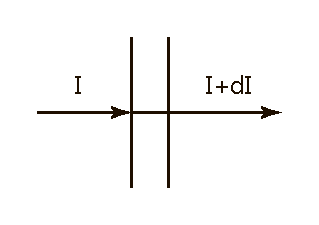
\includegraphics[width=.4\textwidth]{07_01}
	\caption{Пространство со скрещенными полями}
	\label{img07.1}
\end{figure}

Уравнение движения при нерелятивистских скоростях частицы имеет вид
\[
	m_0 \ddot{\vec{R}} = q\vec{E}_0 + q\left[ \vec{v}\vec{B}_0 \right]
\]

Рассмотрим его относительно составляющих по координатам 
\( x \), \( y \), \( z \):
\begin{equation}
	\left. \begin{array}{c}
		\ddot{x} = 0 \\
		\ddot{y} = -\frac{q}{m_0}E_0 + \frac{q}{m_0}B_0 \dot{z} \\
		\ddot{z} = -\frac{q}{m_0}B_0 \dot{y}
	\end{array} \right\}
	\label{eq07.2.65}
\end{equation}

Если частица на входе в систему не имеет составляющей скорости вдоль \( 0x \), 
то ее координата по \( x \) не меняется и траектория будет лежать только в 
плоскости \( у0z \). Для простоты положим, что на влете в систему 
\( x\Big|_{t=0} = 0\), \( \dot{x}\Big|_{t=0} = 0 \), поэтому будем 
рассматривать только два последних уравнения (\ref{eq07.2.65}). Их решение 
можно искать различными путями. Выберем следующий. Проинтегрируем один раз 
по времени последнее уравнение из системы (\ref{eq07.2.65}):
\begin{equation}
	\dot{z} = -\omega_c y + A
	\label{eq07.2.66}
\end{equation}

Если положить начальные условия на влёте частицы в рассматриваемую область в 
виде \( y\Big|_{t=0} = y_0 \), \( z\Big|_{t=0} = 0 \), 
\( \dot{y}\Big|_{t=0} = v_{0y} \), \( \dot{z}\Big|_{t=0} = v_{0z} \), то 
постоянная
\begin{equation}
	A = v_{0z} + \omega_c y_0
	\label{eq07.2.67}
\end{equation}

Подставим полученное решение (\ref{eq07.2.66}) во второе уравнение системы 
(\ref{eq07.2.65}):
\[
	\ddot{y} + \omega^2_c y = -\frac{q}{m_0} E_0 + \omega_c A = 
		-\omega_c u_0 + \omega_c A
\]

где \( u_0 = E_0 / B_0 \) -- переносная скорость электрона. Решение этого 
неоднородного уравнения

\begin{equation}
	y = G\sin\omega_c t + D\cos\omega_c t + \frac{1}{\omega_c}( A - u_0 )
	\label{eq07.2.68}
\end{equation}

а постоянные интегрирования \( D \) и \( G \) определяются из введенных 
начальных условий:

\begin{equation}
	D = y_0 - \frac{1}{\omega_c}( A - u_0 ); \quad
	G = \frac{v_{0y}}{\omega_c}
	\label{eq07.2.69}
\end{equation}

Зависимость \( z(t) \) определим, подставив в (\ref{eq07.2.66}) решение 
(\ref{eq07.2.68}) и проинтегрировав (\ref{eq07.2.66}) по \( t \):
\begin{equation}
	z = G\cos\omega_c t - D\sin\omega_c t + A + C
	\label{eq07.2.70}
\end{equation}

Постоянная интегрирования
\begin{equation}
	C = -G = -\frac{v_{0y}}{\omega_c}
	\label{eq07.2.71}
\end{equation}

Подставляя (\ref{eq07.2.67}), (\ref{eq07.2.69}), (\ref{eq07.2.71}) в выражения 
(\ref{eq07.2.68}) и (\ref{eq07.2.70}), после несложных преобразований 
получаем зависимости \( y(t) \), \( z(t) \):
\begin{equation}
	\left. \begin{array}{c}
		y = y_0 + \frac{v_{0y}}{\omega_c}\sin\omega_c t +
			\frac{u_0-v_{0z}}{\omega_c}(\cos\omega_c t - 1) \\
		z = \frac{v_{0y}}{\omega_c}(\cos\omega_c t - 1 ) - 
			\frac{u_0-v_{0z}}{\omega_c}\sin\omega_c t + u_0 t
	\end{array} \right\}
	\label{eq07.2.72}
\end{equation}

Из (\ref{eq07.2.72}) легко получить параметрическую зависимость
\begin{equation}
	\left[ y - y_0 + \frac{1}{\omega_c}(u_0 - v_{0z}) \right]^2 + 
		\left[ z + \frac{v_{0y}}{\omega_c} - u_0 t \right]^2 = 
		\frac{v^2_{0y} + (u_0 - v_{0z})^2}{\omega^2_c}
	\label{eq07.2.73}
\end{equation}
из которой следует, что частица в скрещенных статистических полях движется по 
окружности с радиусом
\begin{equation}
	R = \frac{1}{|\omega_c|}\sqrt{v^2_{0y}+(u_0 -v_{0z})^2}
	\label{eq07.2.74}
\end{equation}
вокруг центра с изменяющимися во времени координатами:
\begin{equation}
	\left. \begin{array}{c}
		y = y_0 - \frac{1}{\omega_c}(u_0 - v_{0z}) \\
		z = u_0 t - \frac{v_{0z}}{\omega_c}
	\end{array} \right\}
	\label{eq07.2.75}
\end{equation}
Центр окружности перемещается вдоль оси \( 0z \) с постоянной скоростью 
\( u_0 \).

Из (\ref{eq07.2.72}) или (\ref{eq07.2.73}) можно выделить ряд интересных 
частных случаев. 

1. Пусть \( y_0 = v_0 = v_{0z} = 0 \). Тогда
\begin{equation}
	\left. \begin{array}{c}
		y = \frac{u_0}{\omega_c}(\cos\omega_t - 1) \\
		z = \frac{u_0}{\omega_c}(\omega_c t - \sin\omega_c t)
	\end{array} \right\}
	\label{eq07.2.76}
\end{equation}

Система (\ref{eq07.2.76})  описывает циклоиду  (рис.~\ref{img07.2}), 
представляющую собой след точки, лежащей на ободе колеса радиуса 
\( R_\text{окр} = u_0 / \omega_c \), катящегося вдоль оси \( 0z \) со 
скоростью \( u_0 \). На рис.~\ref{img07.2} тонкой пунктирной линией 
нарисована траектория частицы с отрицательным зарядом (\( q < 0 \), 
\( \omega_c < 0 \)). При \( q > 0 \) картина будет иметь такой же вид, если 
изменить знаки у \( E_0 \) и \( B_0 \). Очевидно, что при выполнении условия 
\( d = 2u_0/\omega_c \) частица попадает на верхнюю плоскость. Это условие, 
приводящее к соотношению
\[
	B_{0\text{кр}} = \frac{1}{d}\sqrt{2\left| \frac{m_0}{q} \right| U_0}
\]
определяет критическую величину магнитной индукции, при которой еще возможна 
циклоидальная траектория частицы.

\begin{figure}[h!]
	\center
	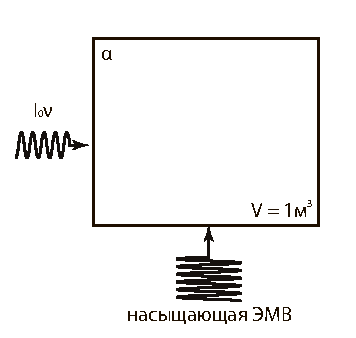
\includegraphics[width=.4\textwidth]{07_02}
	\caption{Траектории частиц в скрещенных полях: \\
		\( \cdot \cdot \cdot \) уравнение (\ref{eq07.2.76}); -- -- уравнение
		(\ref{eq07.2.77}); --- уравнение (\ref{eq07.2.78})}
	\label{img07.2}
\end{figure}

2. Интересен случай, когда \( y = 0 \), \( v_{0y} = 0 \), \( v_{0z} = u_0 \) 
то есть частица влетает в область параллельно плоскостям со скоростью 
\( u_0 \). В этом случае из (\ref{eq07.2.72}) находим:

\begin{equation}
	y = y_0; \quad
	z = u_0 t
	\label{eq07.2.77}
\end{equation}
то есть траектория частицы представляет собой прямую линию. Это соответствует 
случаю, когда частица находится в центре колеса (штриховая линия 
на рис.~\ref{img07.2}).

3. В случае, когда \( v_{0y} = 0 \), а \( v_{0z} \neq u_0\), из 
(\ref{eq07.2.78}) следует, что
\begin{equation}
	\left. \begin{array}{c}
		y = \frac{u_0-v_{0z}}{\omega_c}(\cos\omega_c t - 1) \\
		z = ut - \frac{u_0-v_{0z}}{\omega_c}\sin\omega_c t
	\end{array} \right\}
	\label{eq07.2.78}
\end{equation}
и траектория частицы представляет собой трохоиду (кривая, нарисованная 
сплошной линией на рис.~\ref{img07.2}).

\chapter{Переменные Лагранжа и Эйлера для описания движения частицы сплошной
среды. Вектор смещения. Тензор смещения как сумма тензора деформации и тензора
поворота.}

Лагранж предложил выделить в сплошной среде отдельные точки и следить за их
движением. Координаты которыми характеризуется данная точка и не меняются при
её движении носят название \emph{переменных Лагранжа}. В качестве таких
координат можно выбрать положения точки в начальный момент времени \( \xi^i \)
или её цвет если все точки сплошной среды окрашены в разные цвета.
Закон движения каждой точки в переменных Лагранжа имеет вид
\[
    \vec{r} = \vec{r}(\xi^i, t)
\] 
или в контрвариантных криволинейных координатах \( q^j \)
\[
    q^j = q^j(\xi^i, t).
\]
Скорость по Лагранжу -- скорость движения данной частицы, для неё
\( \xi^i~=~const \):
\[
    \left.\der{\vec{r}}{t}\right|_{\xi^i = const} = \pder{\vec{r}}{t}.
\]
Ускорение по Лагранжу   
\[
    \left.\dder{\vec{r}}{t}\right|_{\xi^i = const} = \ppder{\vec{r}}{t}.
\]
        
Эйлер предложил не следить за каждой отдельной частицей, а следить за данной
точкой пространства измеряя скорости, пролетающих через неё частиц и фиксируя
их вид. Криволинейные координаты данной точки \( q^j \)  и время \( t \) носят
название \emph{переменных Эйлера}.

Выражение для радиус-вектора частицы \( \vec{r} = \vec{r}(\xi^i, t) \) и
компонент радиус-вектора частицы \( q^j = q^j (\xi^i, t) \) позволяет выяснить,
какие частицы проходят через данную точку: \( \xi^i = \xi^i(q^j, t) \).
Скорость по Эйлеру -- скорость в данной точке \( \vec{r}_{M} \):
\[
    \der{\vec{r}}{t} = 
    \left.\pder{\vec{r}}{t}\right|_{\xi^i = \xi^i(\vec{r}_{M}, t)} +
    \left.\pder{\vec{r}}{\xi^i}
    \der{\xi^i}{t}\right|_{\xi^i = \xi^i(\vec{r}_{M}, t)} =
    \left.\pder{\vec{r}}{t}\right|_{\xi^i = \xi^i(\vec{r}_{M}, t)} +
    \left.\pder{\vec{r}}{\xi^i}
    \pder{\xi^i}{t}\right|_{\xi^i = \xi^i(\vec{r}_{M}, t)}
\]
Ускорение по Эйлеру
\[
    \dder{\vec{r}}{t}.
\]

Также иногда вводят перемещение по Эйлеру. \emph{В курсе Лурье} это разность
между конечным и начальным радиус-вектором. Определяя переменные Лагранжа как
координаты радиус-вектора в начальный момент времени и полагая, что наша
система координат не связана с точками сплошной среды (а бывает и такое), для
перемещений по Эйлеру можно записать: \( s^i = q^i - \xi^i \).
    
Рассмотрим две близкие частицы сплошной среды \( A \) и \( B \) в момент
времени \( t \), в следующий момент времени \( t+dt \) они сместятся на
некоторые векторы \( \vec{s}_{A} \), \( \vec{s}_{B} \):
\begin{gather*}
    \vec{s}_{A} = \vec{r}_{A}(t+dt) -\vec{r}_{A}(t),\\
    \vec{s}_{B} = \vec{r}_{B}(t+dt) -\vec{r}_{B}(t).
\end{gather*}
Полагая что координаты вектора \( \vec{r}_{B} - \vec{r}_{A} \) равные в
криволинейных координатах \( \delta q^i \) малы, в первом приближении:
\[
    \vec{s}_{B} - \vec{s}_{A} = \pder{ \vec{s}_{A}}{q^i}\delta q^i 
    = \nabla_i s^j \delta q^i,
\]
\( s^j \) контрвариантные компоненты вектора \( \vec{s}_{A} \).

Вектор \( s^j \) носит название \emph{вектора смещения}. Он показывает, как
сместилась бы частица при поступательном движении будь она частицей твёрдого
тела.

\emph{Тензором смещения} называется тензор \( b^j_{i} = \nabla_i s^j \) или
соответствующий ему ковариантный тензор \( b_{ki} = g_{jk}\nabla_i s^j \).
Тензор смещения можно представить, как и всякий тензор второго ранга, в виде
суммы симметричного и антисимметричного тензоров:
\[
    b^j_{i} = 
    \underbrace{\frac{1}{2} (b^j_{i}+b^j_{i})}_{\substack{= e^j_{i} \\
    \text{симметричный}
    }} \ \ \ + 
    \underbrace{\frac{1}{2} (b^j_{i}-b^j_{i}).}_{\substack{= \phi^j_{i}\\
    \text{антисимметричный}
    }}
\]
Тогда 
\[
    s^j_B = s^j_A + e^j_{i}\delta q^i + \phi^j_{i}\delta q^i.
\]
\sidefig(7cm)
{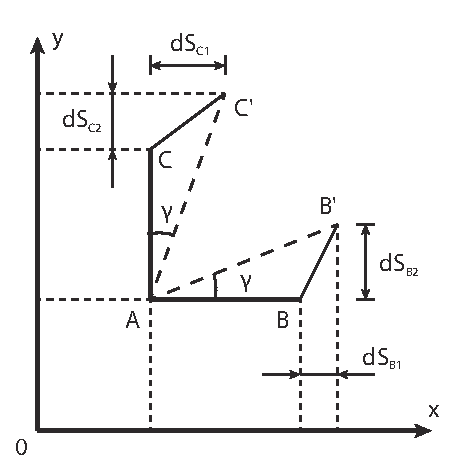
\includegraphics[width=\textwidth]{08}}
{Определим физический смысл тензоров \( e^j_{i} \), \( \phi^j_{i} \).
Рассмотрим плоскую сплошную среду в декартовых координатах \( (x, y) \) или
\( (x^1, x^2) \) как показано на рисунке справа. Выделим в ней два бесконечно
малых стержня \( AB \) и \( AC \). Декартову систему координат привяжем к точке
\( A \) и рассмотрим малые по сравнению со стержнями перемещения точек \( B \)
и \( C \) в точки \( B' \) и \( C' \).}

В декартовых координатах ковариантная производная переходит в частную,
обозначив длины стержней \( AB \) и \( AC \) \( \delta x \) и \( \delta y \)
соответственно, получим:
    \begin{gather*}
    e^1_{1} = \pder{s^1}{x^1} = \frac{ds_{_{B1}}}{\delta x} 
    \text{   - относительная деформация стержня AB,} \\
    e^1_{2} = \pder{s^1}{x^2} = \frac{ds_{_{C1}}}{\delta y} 
    \text{   - поворот(сдвиг) стержня AB на }\gamma, \\
    e^2_{1} = \pder{s^2}{x^1} = \frac{ds_{_{B2}}}{\delta x} 
    \text{   - поворот(сдвиг) стержня AC на }\gamma, \\  
    e^2_{2} = \pder{s^2}{x^2} = \frac{ds_{_{C2}}}{\delta y} 
    \text{   - относительная деформация стержня AC.}
    \end{gather*}
    
Таким образом тензор \( e^j_{i} \) - \textit{тензор деформации}.

Тензор \( \phi^j_{i} \) - антисимметричный, поэтому свёртку
\( \phi^j_{i}\delta q^i \) можно заменить векторным произведением:
\[
    \phi^j_{i}\delta q^i = \vec{\Phi} \times \delta\vec{s}.
\]
Если вспомнить понятие вектора поворота, видно, что это \( \vec{\Phi} \).
Тензор \( \phi^j_{i} \) носит название \emph{тензора поворота}.

\textbf{Теорема Гельмгольца}\\
\textit{Движение малой частицы среды в каждый момент времени представляет
собой поступательное движение вместе с полюсом (точкой внутри малой частицы),
сферическое движение вокруг полюса и движение деформации.}

\newpage

\renewcommand{\labelenumi}{\Roman{enumi}}

\question{Основные законы динамики материальной точки. Законы Ньютона.
Дифференциальные уравнения движения материальной точки. Две основные задачи
динамики точки.}

В основе динамики материальной точки лежат три закона Ньютона:
\begin{enumerate}
    \item закон Ньютона (закон инерции):

    всякое тело сохраняет состояние покоя или равномерного прямолинейного
    движения, пока и поскольку приложенные силы не заставят его изменить это
    состояние;
    
    \item закон Ньютона:

    изменение движения пропорционально приложенной движущей силе и происходит
    в направлении линии действия этой силы;

    \item закон Ньютона:
    
    действию всегда соответствует равное ему и противоположно направленное
    противодействие, то есть действия двух тел друг на друга всегда равны и
    направлены в противоположные стороны.

\end{enumerate}
\renewcommand{\labelenumi}{\arabic{enumi}.}

Эти три закона предполагают существование ``абсолютного времени'' и установлены
для движений материальной точки по отношению к ``абсолютно неподвижной'' системе
координат, а согласно принципу Галилея -- и по отношению к любой инерциальной
(галилеевой) системе отсчета.

\emph{Дифференциальное уравнение движения} материальной точки в векторном виде:
\[
    m\dder{\vec{r}}{t} = \vec{F}.
\]

\subquestion{Две основные задачи динамики материальной точки:}
\emph{Первая задача} (прямая задача):
    
дано движение материальной точки заданной массы, то есть известны координаты
точки как функции времени -- кинематические уравнения движения; требуется найти
силу, действующую на точку.

\emph{Вторая задача} (обратная задача):
    
дана сила, приложенная к материальной точке заданной массы; требуется найти
движение точки, то есть кинематические уравнения движения.

\newpage

\emph{10. Магнетизм атомов. Опыты Штерна и Герлаха. Магнитно-механические 
эффекты. Спин электрона. Квантовые числа электрона и тонкая структура 
спектральных термов. Правила отбора. Понятие об уравнении Дирака.}

\newpage

\chapter{Многоэлектронные атомы. Векторная модель многоэлектронного 
атома. Магнитный момент многоэлектронного атома. Фактор Ланде.}

Механический и магнитный моменты связаны гиромагнитным отношением, но в случае
спиновых моментов, это отношение в два раза больше:
\[
    \mu_L = -\mu_\emph{Б}\sqrt{L(L+1)}, \quad \mu_S = -2\mu_\emph{Б}
    \sqrt{S(S+1)}, \quad \mu_J = -\mu_\emph{Б}g\sqrt{J(J+1)},
\]
где
\[
    g = 1 + \frac{J(J+1) + S(S+1) - L(L+1)}{2J(J+1)} \text{ -- фактор Ланде}.
\]

\section{Векторная модель многоэлектронного атома}

Из-за удвоенного магнетизма спина, \( \mu_J \) начинает прецессировать вокруг
оси, совпадающей с осью, проходящей через \( \vec{M}_J \):

\begin{gather*}
    \average{\mu_{J_z}} = -|\mu_L|\cos\alpha - |\mu_S|\cos\beta; \\
    |\mu_L| = \mu_\emph{Б}\sqrt{L(L+1)}, \quad |\mu_S| = 2\mu_\emph{Б}
    \sqrt{S(S+1)};\\
    M_S^2 = M_L^2 + M_J^2 - 2M_L M_J\cos\alpha, \quad \cos\alpha =
    \frac{-M_S^2 + M_L^2 + M_J^2}{2M_L M_J} = \frac{L(L+1) + J(J+1) - S(S+1)}
    {2\sqrt{L(L+1)}\sqrt{J(J+1)}}; \\
    M_L^2 = M_J^2 + M_S^2 - 2M_J M_S\cos\beta, \quad \cos\beta =
    \frac{M_J^2 + M_S^2 - M_L^2}{2M_S M_J} = \frac{J(J+1) + S(S+1) - L(L+1)}
    {2\sqrt{J(J+1)}\sqrt{S(S+1)}}; \\
    \average{\mu_{J_z}} = -\mu_\emph{Б}\frac{L(L+1) + J(J+1) - S(S+1)}
    {2\sqrt{J(J+1)}} - 2\mu_\emph{Б}\frac{J(J+1) + S(S+1) - L(L+1)}
    {2\sqrt{J(J+1)}}; \\
    \average{\mu_{J_z}} = - \mu_\emph{Б}\frac{3J(J+1) + S(S+1) - L(L+1)}
    {2\sqrt{J(J+1)}} = -\mu_\emph{Б}g\sqrt{J(J+1)} = \mu_J.
\end{gather*}

\begin{figure}[h!]
    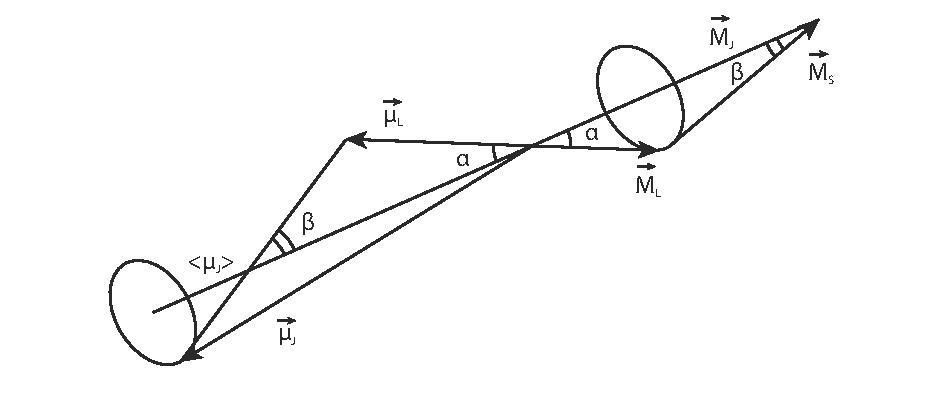
\includegraphics[width=.5\textwidth]{11_01}
\end{figure}

\newpage

\chapter{Ряд Фурье и его коэффициенты. Теорема Дирихле. Дискретный частотный
спектр периодической функции. Преобразование Фурье.}

\section{Ряд Фурье}
Функциональный ряд вида
\[
    \frac{a_0}{2} + \sum\limits_{n=1}^\infty \Bigl(a_n\cos nx + b_n\sin nx\Bigr)
\]
называется тригонометрическим рядом, а постоянные числа \( a_0 \), \( a_n \) и
\( b_n \) \( (n \in \mathcal{N}) \) -- коэффициентами тригонометрического ряда.
Если такой ряд сходится, то его сумма -- периодическая функция с периодом
\( 2\pi \).

Пусть функция \( f(x) \) такова, что она представляется тригонометрическим рядом
на интервале \( (-\pi, \pi) \), то есть
\[
    f(x) = \frac{a_0}{2} + \sum\limits_{n=1}^\infty \Bigl(a_n\cos nx +
    b_n\sin nx\Bigr).
\]
Предположим, что интеграл от функции равен сумме интегралов от членов ряда
(это возможно, если ряд мажорируем, то есть абсолютно сходится ряд
коэффициентов). Интегрируя левую и правую часть от \( -\pi \) до \( \pi \)
имеем:
\[
    \int\limits_{-\pi}^\pi f(x)\d x = \int\limits_{-\pi}^\pi \frac{a_0}{2}\d x +
    \sum\limits_{n=1}^\infty \left(a_n\int\limits_{-\pi}^\pi \cos nx\d x + b_n
    \int\limits_{-\pi}^\pi \sin nx\d x\right) = \pi a_0 \Rightarrow
    a_0 = \frac{1}{\pi}\int\limits_{-\pi}^\pi f(x) \d x.
\]

Домножив обе части на \( \cos mx \) и проинтегрировав, получим:
\[
    a_m = \frac{1}{\pi} \int\limits_{-\pi}^\pi f(x)\cos mx\d x.
\]
Проводя аналогичные действия с \( \sin mx \), получим:
\[
    b_m = \frac{1}{\pi} \int\limits_{-\pi}^\pi f(x)\sin mx \d x.
\]

Коэффициенты, определённые по этим формулам, называются коэффициентами Фурье
функции \( f(x) \), а тригонометрический ряд с такими коэффициентами -- рядом
Фурье функция \( f(x) \).

\section{Теорема Дирихле}
Если \( f(x) \) -- ограниченная периодическая функция, имеющая на каждом периоде
конечное число максимумов, минимумов и точек разрыва, то ряд Фурье функции
\( f(x) \) сходится к \( f(x) \) в каждой точке непрерывности функции и к
среднему арифметическому пределов функции слева и справа в точке разрыва.

\section{Дискретный частотный спектр периодической функции}
Если \( f(x) \) -- периодическая функция, то разложение в ряд Фурье можно
интерпретировать как сопоставление функции \( f(x) \) последовательности
\( \{c_n\} \), где \( c_n = \sqrt{a_n^2 + b_n^2} \).

\section{Преобразование Фурье}
Рассмотрим непериодическую функцию \( f(x) \), определенную на \( (-\infty,
\infty) \) и абсолютно интегрируемую на нём. Тогда в пределе \( l \to \infty \)
можно перейти от ряда Фурье на конечном отрезке \( [-l, l] \) к интегралу Фурье:
\[
    f(x) = \int\lni a(\xi)\cos(\xi x)\d\xi + \int\lni b(\xi)\sin(\xi x)\d\xi,
\]
где \( \ds a(\xi) = \frac{1}{\pi} \int\limits_{-\infty}^{+\infty}
f(x)\cos(\xi x)\d x \), \( \ds b(\xi) = \frac{1}{\pi}
\int\limits_{-\infty}^{+\infty} f(x)\sin(\xi x)\d x \).

Если учесть, что \( \ds \sin x = \frac{\e^{\i x} - \e^{-\i x}}{2\i} \), а
\( \ds \cos x = \frac{\e^{\i x} + \e^{-\i x}}{2} \), то можно записать
комплексный вид интеграла Фурье:
\[
    f(x) = \frac{1}{2\pi}\int\limits_{-\infty}^{+\infty} \left[
    \int\limits_{-\infty}^{+\infty} f(x)\cdot\e^{-\i\xi x}\d x\right]
    \e^{\i\xi x}\d\xi.
\]

Отсюда получаем пару интегральных преобразований:
\[
    F[f] = F(\xi) = \frac{1}{\sqrt{2\pi}}\int\limits_{-\infty}^{+\infty} f(x)
    \e^{-\i\xi x}\d x, \quad
    F^{-1}[F] = f(x) = \frac{1}{\sqrt{2\pi}}\int\limits_{-\infty}^{+\infty} f(x)
    \e^{\i\xi x}\d\xi.
\]
\newpage

\chapter{Свойства преобразования Фурье. Решение задачи о распространении тепла
в бесконечном стержне с заданной начальной температурой.}

Свойства преобразования Фурье:
\begin{enumerate}
    \item обратимость: \( F^{-1}\bigl[F[f]\bigr] = f \);
    \item линейность: \( F[af + bg] = aF[f] + bF[g] \);
    \item преобразование производных:
    \( \ds
        \pnder{n}{u}{x} \to (\i\xi)^n\cdot F_x[u],\ 
        \pnder{n}{u}{t} \to \pnder{n}{}{t} F_x[u];
    \)
    \item свёртка:    
    \( F[f * g] = F[f]\cdot F[g] \), где
    \[ 
        (f * g)(x) = \frac{1}{\sqrt{2\pi}}\int\limits_{-\infty}^{+\infty}
        f(x-\xi)g(\xi)\d\xi = F^{-1}\bigr[F[f]\cdot F[g]\bigl]
        \text{ -- свёртка}.
    \]
\end{enumerate}

\begin{minipage}{.67\textwidth}
    Рассмотрим теперь \emph{задачу о распространении тепла в бесконечном стержне},
    если задана начальная температура \( u(x, 0) = \phi(x) \).

    Сделаем преобразование Фурье по переменной \( x \): \( u \to \bar{u} \).
\end{minipage}
\hfill
\begin{minipage}{.3\textwidth}
    \[
        \left\{ \begin{array}{l}
            \ds \pder{u}{t} = \alpha^2 \ppder{u}{x}; \\
            u(x, 0) = \phi(x).
        \end{array} \right.
    \]
\end{minipage}

\begin{minipage}{.67\textwidth}
    Преобразованная задача:
    
    Её решение: \( \ds \bar{u} = \bar{\phi}(\xi)\cdot\e^{-\alpha^2\xi^2 t} \).
\end{minipage}
\hfill
\begin{minipage}{.3\textwidth}
    \[
        \left\{ \begin{array}{l}
            \ds \pder{u}{t} = \alpha^2 \ppder{u}{x}; \\
            u(x, 0) = \phi(x).
        \end{array} \right.
    \]
\end{minipage}

Обратным преобразованием Фурье получаем ответ:
\[
    u(x, t) = F^{-1}[\bar{\phi}(\xi)\cdot\e^{-\alpha^2\xi^2 t}] =
    F^{-1}[\bar{\phi}(\xi)] * F^{-1}[\e^{-\alpha^2\xi^2 t}] =
    \frac{1}{2\alpha\sqrt{\pi t}} \int\limits_{-\infty}^{+\infty} \phi(s)
    \e^{\frac{-(x-s)^2}{4\alpha^2 t}}\d s.
\]

Функция \( \ds G(x, t) = \frac{1}{2\alpha\sqrt{\pi t}}
\e^{\frac{-x^2}{4\alpha^2 t}} \) называется функцией Грина. Тогда ответ
может быть представлен в виде:
\[
    u(x, t) = \int\limits_{-\infty}^{+\infty} \phi(s)\cdot G(x-s, t)\d s.
\]

\newpage

\question{Матрица плотности}
\chapter{Действие для частиц и поля (общая форма записи).}

\section{Действие для частиц и поля (общая форма записи)}

\question{Основные законы (теоремы) механики для материальной точки. Теорема об
изменении момента импульса (момента количества движения, кинетического
момента). Закон сохранения момента импульса.}

Основными теоремами механики материальной точки являются:
\begin{enumerate}
    \item теорема об изменении количества движения (и соответствующий ей закон
    сохранения импульса);
    \item теорема об изменении момента количества движения (и соответствующий ей
    закон сохранения момента импульса);
    \item теорема об изменении кинетической энергии.
\end{enumerate}

\subquestion{Теорема об изменении момента импульса}

Запишем основное уравнение динамики: \( \ds m\der{\vec{v}}{t} = \vec{F} \) и
умножим его векторно на радиус-вектор точки \( \vec{r} \), определяющий положение
материальной точки относительно какой-либо точки \( O \), которую будем называть
центром:
\[
    \vec{r}\times m\der{\vec{v}}{t} = \vec{r}\times\vec{F}.
\]
Заметим, что
\[
    \der{}{t}(\vec{r}\times m\vec{v}) = \der{\vec{r}}{t}\times m\vec{v} +
    \vec{r}\times m\der{\vec{v}}{t} = \vec{v}\times m\vec{v} +
    \vec{r}\times m\der{\vec{v}}{t} = \vec{r}\times m\der{\vec{v}}{t},
\]
откуда
\[
    \der{}{t}(\vec{r}\times m\vec{v}) = \vec{r}\times\vec{F}.
\]

Вектор \( \vec{k}_O = \vec{r}\times m\vec{v} \) называется моментом количества
движения материальной точки относительно центра (точки \( O \)). Вектор
\( \vec{m}_O = \vec{r}\times\vec{F} \) -- момент приложенной к точке силы
относительно центра.

Таким образом: \( \ds \der{\vec{k}_O}{t} = \vec{m}_O \). Это уравнение выражает
теорему об изменении момента количества движения материальной точки: производная
по времени от момента количества движения материальной точки относительно
какого-либо центра равна моменту силы, приложенной к точке, относительно того же
центра.

\subquestion{Закон сохранения момента импульса}

Если сумма моментов приложенных сил равна нулю \( \sum\vec{m}_{O_k} = 0 \),
то момент количества движения постоянен \( \vec{k}_O = \const \).

\newpage % ---------------------------------------------------------------------

\chapter{Уравнение колебаний струны и его интуитивная интерпретация.
Замечания.}

\newpage

\chapter{Решение одномерного волнового уравнения с помощью формулы д'Аламбера.
Примеры применения формулы д'Аламбера в некоторых конкретных задачах.}

Начнём с решения задачи Коши:
\begin{align*}
    \ppder{u}{t} = c^2\ppder{u}{x}, \quad x\in\mathbb{R},\ t > 0, \\
    \left\{ \begin{array}{l}
        u(x, 0) = \phi(x), \\
        \ds \pder{u}{t}(x, 0) = \psi(x).
    \end{array} \right.
\end{align*}

Уравнение \( \ds \ppder{u}{t} - c^2\ppder{u}{x} = 0 \) является уравнением
гиперболического типа. Приведем его к каноническому виду. Уравнение характеристик
имеет вид: \( \d x^2 - c^2\d t^2 = 0 \), и далее:
\[
    \left[ \begin{array}{l}
        \d x - c\d t = 0 \\
        \d x + c\d t = 0
    \end{array} \right.
    \quad\Leftrightarrow\quad
    \left[ \begin{array}{l}
        x - ct = C_1 = \xi \\
        x + ct = C_2 = \eta
    \end{array} \right.
\]

В координатах \( \xi \) и \( \eta \) уравнение приобретает канонический вид:
\( \ds \pcder{u}{\xi}{\eta} = 0 \).
Дважды проинтегрировав его, найдем, что \( u = f(\xi) + g(\eta) =
f(x - ct) + g(x + ct) \).

Теперь воспользуемся начальными условиями:
\[
    \left\{ \begin{array}{l}
        f(x) + g(x) = \phi(x), \\
        -cf'(x) + cg'(x) = \psi(x),
    \end{array} \right.
    \quad\Leftrightarrow\quad
    \left\{ \begin{array}{l}
        f(x) + g(x) = \phi(x), \\
        \ds -f(x) + g(x) = \frac{1}{c}\int\limits_{x_0}^x\psi(\zeta)\d\zeta + K.
    \end{array} \right.
\]

\begin{align*}
    \text{Отсюда, }\quad & f(x) = \frac{1}{2}\phi(x) -
    \frac{1}{2c}\int\limits_{x_0}^x \psi(\zeta)\d\zeta - \frac{K}{2}, \\
    & g(x) = \frac{1}{2}\phi(x) + \frac{1}{2c}\int\limits_{x_0}^x
    \psi(\zeta)\d\zeta + \frac{K}{2}.
\end{align*}

Тогда решение имеет вид
\[
    u(x, t) = \frac{1}{2}\bigl[\phi(x - ct) + \phi(x + ct)\bigr] + \frac{1}{2c}
    \int\limits_{x - ct}^{x + ct} \psi(\zeta)\d\zeta.
\]

Полученное выражение называется формулой д'Аламбера.

\section{Примеры применения формулы д'Аламбера}
\begin{enumerate}
    \item Рассмотрим начальные условия вида 
    \[
        \left\{ \begin{array}{l}
            u(x, 0) = \sin x, \\
            \ds \der{u}{t}(x, 0) = 0.
        \end{array} \right.
    \]
    
    По формуле д'Аламбера получаем решение:
    \[
        u(x, t) = \frac{1}{2}\bigl(\sin(x - ct) + \sin(x + ct)\bigr),
    \]
    которое можно интерпретировать так: начальное смещение струны
    \( u(x, 0) = \sin x \) делится на две одинаковые части, и каждая из частей
    распространяется со скоростью \( c \) в виде бегущих волн.
    Одна из волн перемещается слева направо, а вторая -- в противоположном
    направлении.
    
    \item Рассмотрим начальные условия вида 
    \[
        \left\{ \begin{array}{l}
            u(x, 0) = 0, \\
            \ds \der{u}{t}(x, 0) = \sin x.
        \end{array} \right.
    \]
    
    По формуле д'Аламбера получаем решение:
    \[
        u(x, t) = \frac{1}{2c}\int\limits_{x - ct}^{x + ct} \sin\zeta\d\zeta =
        \frac{1}{2}\bigl(\cos(x - ct) - \cos(x + ct)\bigr),
    \]
    представляющее собой сумму двух бегущих косинусоидальных волн.
\end{enumerate}

\newpage

\end{document}
